\chapter{Herramientas Utilizadas}
\label{cap:herramientas}

En este capítulo se van a explicar las herramientas utilizadas para el desarrollo de este trabajo. En el apartado 3.1 se explicará Django que es el \textit{framework} utilizado para el desarrollo de la aplicación y en el apartado 3.2 se explicará SpaCy, que es la herramienta que se ha utilizado para la clasificación semántica de las palabras. 


%-------------------------------------------------------------------
\section{Django}
%-------------------------------------------------------------------
\label{cap:sec:django}
Para construir un servicio web se necesita una manera de gestionar los elementos propios de estos servicios\footnote{https://tutorial.djangogirls.org/es/django/}. Algunos de estos elementos son el procesamiento de formularios y el mapeo de urls, que requieren \textit{frameworks} web\footnote{estructuras que contienen los componentes necesarios para el desarrollo de aplicaciones web} para su gestión. 
Django es un \textit{framework} de alto nivel que permite el desarrollo rápido de sitios web seguros y mantenibles y se basa en el patrón MVC\footnote{https://docs.djangoproject.com/en/2.0/}. Fue desarrollado entre los años 2003 y 2005 por un grupo de programadores que se encargaban de crear y mantener sitios web de periódicos. 
Es gratuito y de código abierto y dispone de una gran documentación actualizada así como muchas opciones de soporte gratuito y de pago. 

Algunas de las razones por las que se ha elegido este \textit{framework} han sido las siguientes\footnote{https://openwebinars.net/blog/que-es-django-y-por-que-usarlo/}:

\begin{itemize}
	\item Seguridad: Implementa por defecto algunas medidas de seguridad para evitar SQL Injection (adición de consultas SQL malignas que puedan alterar la base de datos) o Clickjacking (que el usuario haga click en un enlace oculto, para obtener información del mismo sin su permiso o incluso tomar el control de su ordenador).
	
	\item Escalabilidad: Se puede pasar de una aplicación sencilla a otra más compleja rápidamente, ya que es muy fácil añadir nuevos módulos al \textit{framework}.
	
	\item Fácil acceso a bases de datos mediante ORM\footnote{biblioteca para el acceso de datos, generando clases a partir de las tablas de la base de datos para poder realizar las consultas} (Object Relational Mapper). Django tiene su propio ORM, con el que se pueden hacer consultas de manera muy intuitiva.
	
	\item Popularidad: Django es muy popular, por lo que hay mucha documentación disponible y muchos hilos en foros de programación en donde encontrar soluciones para cualquier problema que surja.
	
\end{itemize}



\section{SpaCy}
\label{cap:sec:spacy}
Dentro de las palabras relacionadas con el concepto introducido por el usuario, solo nos interesan los nombres, verbos y adjetivos. Para identificar estas categorías léxicas se necesita un analizador léxico. En nuestro trabajo hemos usado SpaCy\footnote{https://spacy.io/}, que es una biblioteca de código abierto para el Procesamiento del Lenguaje Natural en Python que soporta más de 34 idiomas, entre ellos el español.



%\figura{Bitmap/Capitulo3/spacy}{width=.8\textwidth}{fig:spacy}{Ejemplo de clasificación de palabras}

El analizador semántico de SpaCy, según un estudio realizado en 2015 por la universidad Emory\footnote{https://www.aclweb.org/anthology/P15-1038}, es el más rápido y según Medium Corporation tiene un índice de acierto mucho mayor que el analizador sintáctico de NLTK(que era la alternativa a SpaCy que se estudió) \footnote{https://medium.com/@pemagrg/private-nltk-vs-spacy-3926b3674ee4}.Para utilizar el analizador, hay que importar la biblioteca de idioma correspondiente (en este caso español: ``es\_core\_news\_sm'') y pasar como parámetro las palabras que se deseen clasificar. El resultado para cada palabra introducida en el analizador, serán una serie de etiquetas, de todas ellas, la utilizada es la etiqueta ``pos'', que contiene el grupo semántico de la palabra analizada, como se puede ver en la Figura \ref{fig:spacy}, se ha introducido la frase: ``el coche es rojo'' y se han obtenido los siguientes resultados:
\begin{itemize}
	\item el: ha obtenido la etiqueta DET, haciendo referencia a que es un determinante.
	\item coche: ha obtenido la etiqueta NOUN, que significa nombre en inglés.
	\item es: ha obtenido la etiqueta AUX, haciendo referencia a que es un verbo auxiliar.
	\item rojo: ha obtenido la etiqueta ADJ, haciendo referencia a que es un adjetivo.
\end{itemize}

\begin{figure}[!h]
	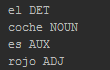
\includegraphics[width=.4\textwidth]{Imagenes/Bitmap/Capitulo3/spacy}
	\centering
	\caption{Ejemplo de clasificación de palabras}
	\label{fig:spacy}
\end{figure}

Inicialmente se utilizó el POS-tagger (clasificador sintáctico de palabras) de NLTK, pero su índice de acierto no era muy bueno, por lo que se descartó su uso. 
